\section{Projekt}

\subsection{Uvod}

Cilj ovog projekta bio je izraditi pristupni modul za infotainment sustav
koji će se koristiti u vozilu Peugeot 206. Sam sustav sastoji se od dvaju glavnih dijelova:
pristupnog modula i računala. Pristupni modul izrađen je pločica vlastitog dizajna
temeljena na modulu ESP32 Wroom 32E. Pločica upravlja napajanjem,
komunikacijom s vozilom te komunikacijom s računalom.
Računalo čini Raspberry Pi 4 sa zaslonom osjetljivim na dodir
(DSI) i prilagođenom Linux distribucijom. Ono upravlja prikazom slike i zvuka.

\bigskip
\noindent
Ovaj projekt je proširenje postojećeg završnog rada `VAN protokol i njegova primjena u automobilima' \cite{mathos-rad}.

\begin{figure}[H]
  \begin{center}
    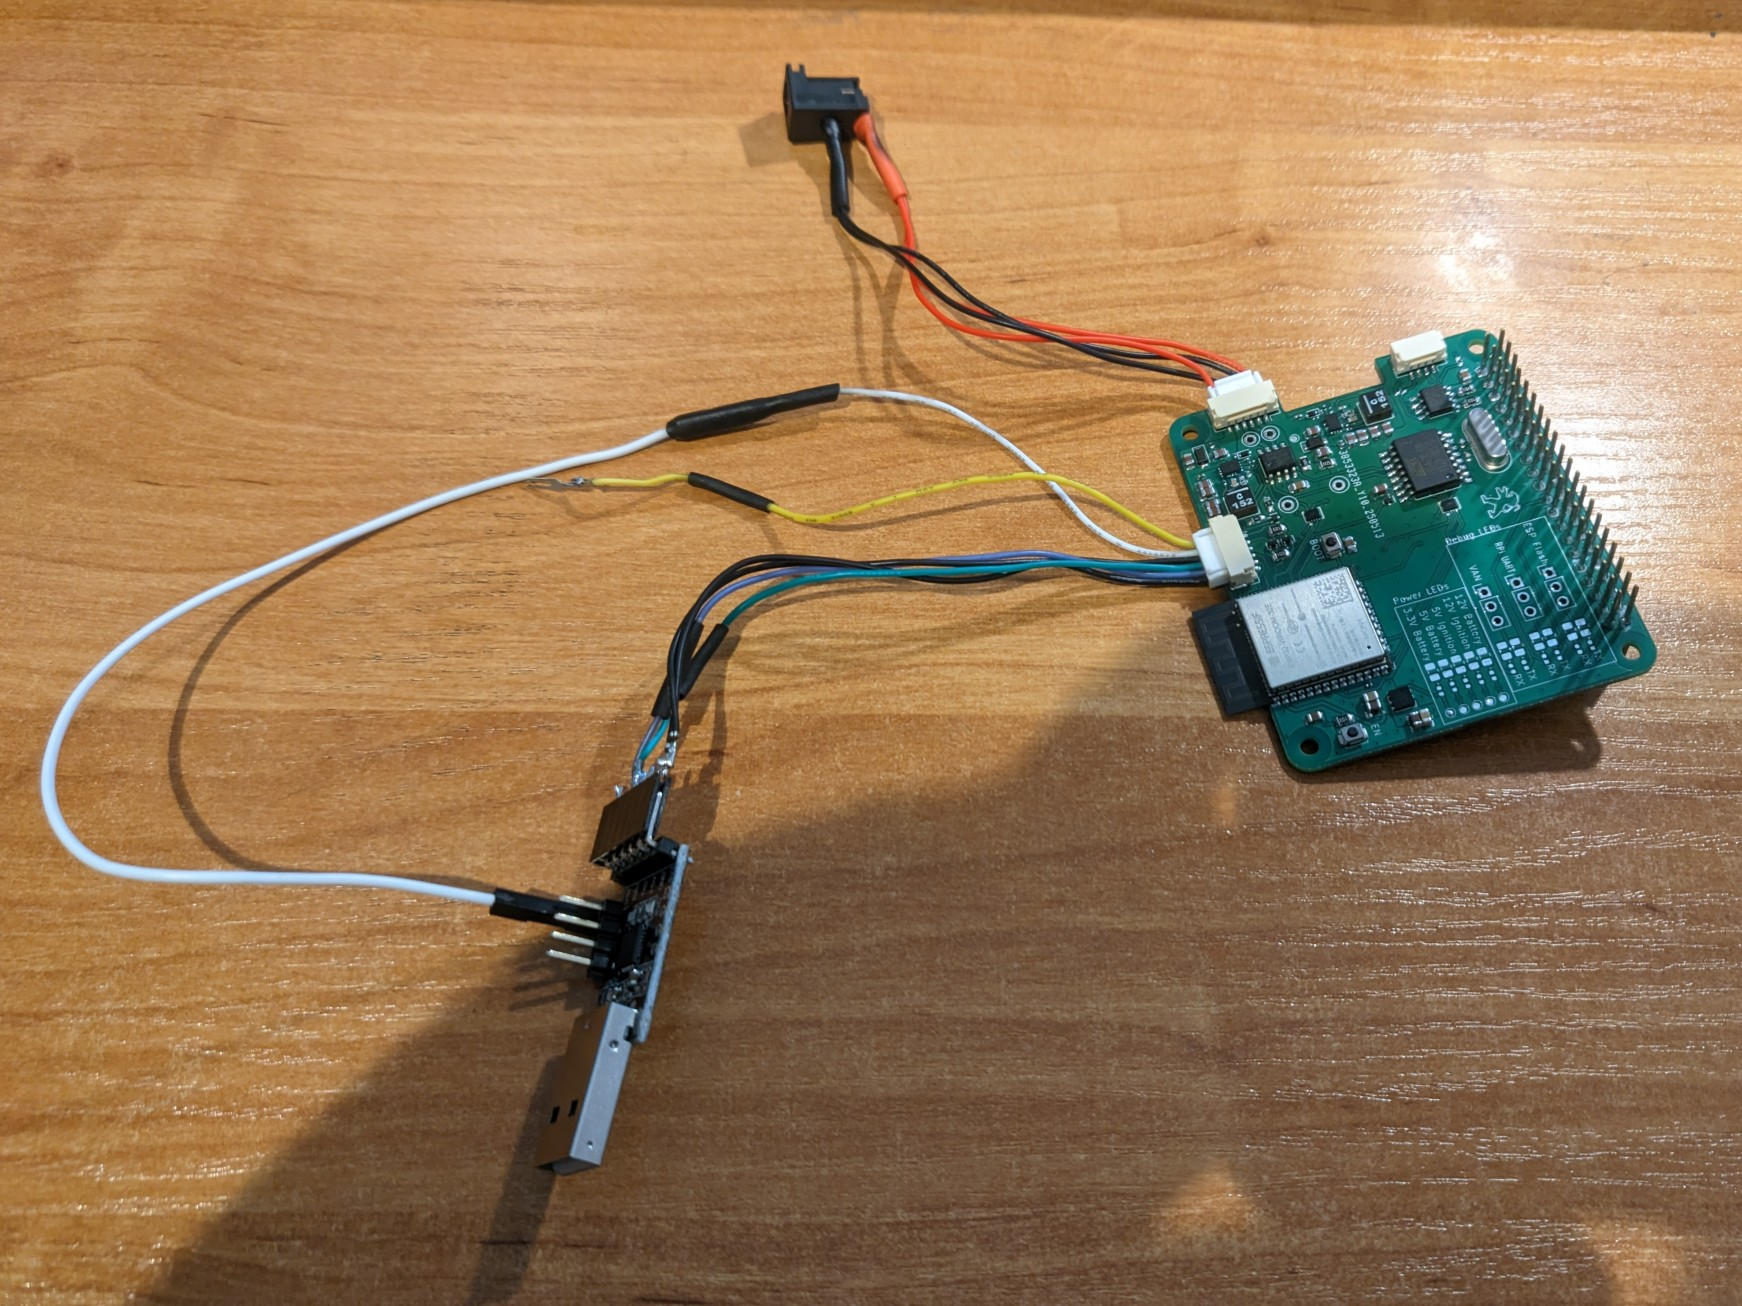
\includegraphics[width=0.75\textwidth]{images/PXL_20250530_205606724.jpg}
    \caption{Izgled pristupnog modula sa sklopovljem za programiranje.}
  \end{center}
\end{figure}

\subsection{Glavni izazovi}

Ovaj projekt ima dva, možda tri glavna izazova koje treba razmotriti. 
Najizraženiji je komunikacija s vozilom. Peugeot 206 ne koristi standardnu CAN sabirnicu, već nešto što se naziva VAN, vidi poglavlje \ref{sec:van_bus}. 
Taj komunikacijski standard danas je zastario, jer je korišten isključivo u vozilima Peugeot i Citroën tijekom ograničenog vremenskog razdoblja. 
Zbog toga gotovo da i ne postoji hardver koji može razumjeti taj protokol, 
a dokumentacije je približno jednako malo, pri čemu je većina napisana na francuskom jeziku. 
Stoga moramo izraditi vlastiti softver za primanje VAN okvira te pronaći način kako ih i slati.

\bigskip
\noindent
Drugi izazov odnosi se na napajanje. 
Imamo komponente koje zahtijevaju i 5 volti i 3,3 volta, kao i dva naponska voda: trajni izvor i uključivi izvor. 
Dodatni problem je \textbf{vrlo} šumovito i ponekad nestabilno ulazno napajanje, pa jeftini istosmjerni pretvarači (DC-DC) neće biti dovoljni.

\bigskip
\noindent
Posljednji izazov, a možda i najpodcijenjeniji, 
jest izrada pouzdane programske podrške (eng. \textit{firmwarea}) za sam pristupni modul. 
Modul ne treba samo analizirati VAN okvire, već mora upravljati vlastitim stanjem, pratiti stanje vozila, upravljati napajanjem i komunikacijom 
računala, kontrolirati režime mirovanja i upravljati vlastitim niskonaponskim stanjem, te, što je najvažnije, ne smije dolaziti do pada sustava.